% [NEW]: Chuong 4 - Ung dung Openlet (viet moi hoan toan)
\chapter{Ứng dụng Openlet}

% [NEW]: Section 4.1 - Gioi thieu ung dung
\section{Giới thiệu ứng dụng}

Nhằm hiện thực hóa các kết quả nghiên cứu từ môi trường học thuật sang một sản phẩm công nghệ giáo dục có giá trị ứng dụng thực tiễn, nghiên cứu đã phát triển ứng dụng Web mang tên Openlet. Ứng dụng này đóng vai trò là nền tảng trực tuyến cho phép giáo viên tạo các bài kiểm tra trắc nghiệm từ ảnh chụp tài liệu học tập, đồng thời cung cấp giao diện để học sinh tham gia làm bài và nhận phản hồi kết quả ngay trên hệ thống.

Đối tượng sử dụng chính của Openlet bao gồm hai nhóm. Nhóm thứ nhất là đội ngũ giáo viên, những người cần nhanh chóng tạo ra các bài kiểm tra trắc nghiệm từ tài liệu giảng dạy hiện có mà không phải tốn nhiều thời gian biên soạn thủ công. Nhóm thứ hai là học sinh, những người tham gia làm bài kiểm tra trực tuyến để ôn tập và củng cố kiến thức.

% [MODIFY]: Loai bo DCP v5, mo ta kien truc chung
% [MODIFY]: Dien dat lai cho tu nhien hon
Openlet tích hợp đầy đủ kiến trúc đa tác tử đã được trình bày chi tiết tại Chương 3. Tuy nhiên, khác với phiên bản nghiên cứu sử dụng vòng lặp thử lại nhiều lần, phiên bản ứng dụng được tối ưu cho trải nghiệm người dùng: mỗi giai đoạn kiểm chứng chỉ thực hiện một lượt duy nhất nhằm rút ngắn thời gian phản hồi. Quy trình hoạt động tổng thể của ứng dụng bắt đầu từ việc người dùng tải lên ảnh chụp hoặc tệp PDF của tài liệu học tập, hệ thống tiến hành trích xuất văn bản thông qua mô hình ngôn ngữ thị giác, phân tích nội dung, sinh câu hỏi trắc nghiệm theo nhiều cấp độ nhận thức Bloom với kiểm chứng chất lượng, và cuối cùng tạo thành một bài kiểm tra trực tuyến kèm giải thích chi tiết.

% [NEW]: Section 4.2 - Kien truc he thong
\section{Kiến trúc hệ thống}

% [NEW]: Subsection 4.2.1 - Kien truc tong quan
\subsection{Kiến trúc tổng quan}

Ứng dụng Openlet được thiết kế theo kiến trúc ba tầng (three-tier architecture), trong đó mỗi tầng đảm nhận một nhóm trách nhiệm riêng biệt nhằm đảm bảo tính mô-đun hóa và khả năng mở rộng của hệ thống.

\textbf{Tầng giao diện (Presentation Tier):} Tầng này chịu trách nhiệm hiển thị và tương tác trực tiếp với người dùng. Ứng dụng sử dụng khung phát triển Next.js kết hợp với thư viện React để xây dựng giao diện theo mô hình ứng dụng trang đơn (Single Page Application). Hệ thống thành phần giao diện được xây dựng dựa trên thư viện Radix UI, cung cấp các thành phần tương tác có khả năng truy cập cao và tuân thủ các tiêu chuẩn về trải nghiệm người dùng. Toàn bộ giao diện được định kiểu thông qua hệ thống thiết kế Tailwind CSS, cho phép phát triển nhanh chóng và duy trì tính nhất quán về mặt thẩm mỹ trên toàn bộ ứng dụng.

% [MODIFY]: Giam bot chi tiet ky thuat, viet khai quat hon
\textbf{Tầng dịch vụ (Service Tier):} Tầng này đóng vai trò trung gian xử lý nghiệp vụ và quản lý dữ liệu. Openlet tận dụng hệ sinh thái Firebase của Google Cloud để triển khai toàn bộ tầng dịch vụ, bao gồm cơ sở dữ liệu hướng tài liệu cho việc lưu trữ và truy vấn dữ liệu, hệ thống lưu trữ đám mây cho các tệp tin tải lên, và các hàm xử lý phía máy chủ thực thi toàn bộ logic nghiệp vụ bao gồm trích xuất văn bản, sinh câu hỏi, chấm điểm và quản lý trạng thái.

% [MODIFY]: Dien dat lai cho phu hop bao cao khoa hoc
\textbf{Tầng trí tuệ nhân tạo (AI Tier):} Tầng này cung cấp năng lực xử lý ngôn ngữ tự nhiên và thị giác máy tính cho hệ thống. Openlet sử dụng cổng trung gian OpenRouter làm điểm truy cập thống nhất, cho phép hệ thống linh hoạt chuyển đổi giữa nhiều mô hình ngôn ngữ khác nhau thông qua cấu hình. Kiến trúc này mang lại lợi thế quan trọng: khi một mô hình mới có hiệu năng tốt hơn hoặc chi phí thấp hơn xuất hiện trên thị trường, người quản trị chỉ cần thay đổi tham số cấu hình thay vì phải tái cấu trúc toàn bộ hệ thống.

% [NEW]: Subsection 4.2.2 - Co so du lieu
\subsection{Cơ sở dữ liệu}

% [MODIFY]: Loai bo ten collection code, dung ngon ngu bao cao
Openlet sử dụng Cloud Firestore, một hệ quản trị cơ sở dữ liệu hướng tài liệu thuộc nền tảng Firebase, để lưu trữ toàn bộ dữ liệu nghiệp vụ. Mô hình dữ liệu được thiết kế xoay quanh bộ sưu tập chính lưu trữ các bài kiểm tra, trong đó mỗi tài liệu đại diện cho một bài kiểm tra và chứa đầy đủ thông tin cần thiết.

Mỗi tài liệu bài kiểm tra bao gồm các nhóm trường dữ liệu sau:

\begin{itemize}
    \item \textbf{Siêu dữ liệu bài kiểm tra:} Các trường lưu trữ thông tin mô tả như tiêu đề, mô tả nội dung, danh sách chủ đề, ngày tạo, định danh người tạo và trạng thái hiện tại của bài kiểm tra.

    \item \textbf{Dữ liệu văn bản gốc:} Văn bản đã được trích xuất từ ảnh hoặc tệp PDF thông qua quy trình nhận dạng ký tự quang học, phục vụ làm nguồn ngữ liệu cho quá trình sinh câu hỏi.

    \item \textbf{Mảng câu hỏi:} Mỗi phần tử trong mảng biểu diễn một câu hỏi trắc nghiệm, bao gồm nội dung câu hỏi, bốn phương án lựa chọn, chỉ số của đáp án đúng, giải thích chi tiết cho đáp án và cấp độ nhận thức Bloom tương ứng.

    \item \textbf{Cấu hình sinh câu hỏi:} Lưu trữ tên mô hình ngôn ngữ được sử dụng và chế độ sinh (chỉ dẫn đơn hoặc đa tác tử), cho phép truy vết và tái tạo kết quả.

    \item \textbf{Thiết lập công khai:} Các trường kiểm soát việc chia sẻ bài kiểm tra, bao gồm trạng thái xuất bản, cho phép người dùng ẩn danh, chính sách cho phép làm lại, cấu hình bộ đếm thời gian và mức độ hiển thị kết quả.

    \item \textbf{Số liệu thống kê:} Các chỉ số tổng hợp được cập nhật tự động sau mỗi lượt nộp bài, bao gồm tổng số lượt làm bài, điểm trung bình, điểm cao nhất, điểm thấp nhất, phân phối điểm theo năm khoảng và danh sách năm người đạt điểm cao nhất.
\end{itemize}

% [MODIFY]: Loai bo ten collection code
Bên cạnh bộ sưu tập chính, mỗi bài kiểm tra còn chứa một bộ sưu tập con lưu trữ dữ liệu bài làm của từng người tham gia. Mỗi tài liệu trong bộ sưu tập con này ghi nhận định danh người làm bài, tên hiển thị, điểm số đạt được, số câu trả lời đúng, tổng số câu hỏi, đáp án đã chọn cho từng câu và thời điểm nộp bài. Cấu trúc bộ sưu tập con này cho phép truy vấn hiệu quả lịch sử làm bài của từng học sinh mà không ảnh hưởng đến hiệu năng đọc dữ liệu bài kiểm tra.

Về mặt lưu trữ tệp tin, Cloud Storage được sử dụng để tiếp nhận tạm thời các tệp ảnh và PDF mà người dùng tải lên. Sau khi quá trình trích xuất văn bản hoàn tất thành công, các tệp tạm thời này được tự động xóa khỏi hệ thống lưu trữ nhằm tối ưu hóa chi phí và dung lượng.

% [NEW]: Subsection 4.2.3 - Xac thuc va bao mat
\subsection{Xác thực và bảo mật}

Hệ thống xác thực của Openlet được xây dựng trên nền tảng Firebase Authentication, hỗ trợ hai phương thức đăng nhập. Phương thức thứ nhất là đăng nhập ẩn danh, cho phép học sinh nhanh chóng tham gia làm bài kiểm tra mà không cần đăng ký tài khoản, phù hợp với các tình huống sử dụng một lần trong lớp học. Phương thức thứ hai là đăng nhập bằng thư điện tử, dành cho giáo viên và những người dùng cần lưu trữ lịch sử hoạt động lâu dài.

Mô hình phân quyền của ứng dụng được thiết kế dựa trên hai vai trò chính. Vai trò \textit{chủ bài kiểm tra} là người đã tạo ra bài kiểm tra, có toàn quyền chỉnh sửa nội dung câu hỏi, quản lý thiết lập công khai, xem toàn bộ đáp án đúng cùng giải thích, truy cập thống kê chi tiết và xóa các lượt làm bài. Vai trò \textit{người làm bài} là học sinh tham gia làm bài kiểm tra, chỉ được phép xem đề bài, nộp bài và nhận kết quả theo mức hiển thị mà giáo viên đã cấu hình.

% [MODIFY]: Thay Cloud Functions bang mo ta chung
Một nguyên tắc bảo mật quan trọng được áp dụng xuyên suốt hệ thống là đáp án đúng không bao giờ được gửi về phía máy khách. Khi người làm bài truy cập đề bài, hệ thống chỉ trả về nội dung câu hỏi và các phương án lựa chọn, trong khi chỉ số đáp án đúng, giải thích và các trường nhạy cảm khác đều được loại bỏ tại tầng máy chủ. Toàn bộ quá trình chấm điểm được thực hiện hoàn toàn phía máy chủ: khi học sinh nộp bài, đáp án được gửi lên để đối chiếu với đáp án đúng lưu trong cơ sở dữ liệu, và chỉ có kết quả đã được lọc theo mức hiển thị mới được trả về cho người dùng.

Cơ chế kiểm soát mức độ hiển thị kết quả cho phép giáo viên tinh chỉnh lượng thông tin phản hồi mà học sinh nhận được sau khi nộp bài, thông qua năm mức hiển thị:

\begin{itemize}
    \item \textbf{Mức 0 - Không hiển thị:} Học sinh không nhận được bất kỳ thông tin phản hồi nào sau khi nộp bài, chỉ biết rằng bài làm đã được ghi nhận.
    \item \textbf{Mức 1 - Hiển thị điểm:} Học sinh chỉ được xem điểm số tổng thể, bao gồm số câu trả lời đúng trên tổng số câu hỏi và phần trăm đạt được.
    \item \textbf{Mức 2 - Hiển thị đúng/sai:} Ngoài điểm số, học sinh còn được biết từng câu hỏi cụ thể đã trả lời đúng hay sai, giúp nhận diện các phần kiến thức cần ôn tập.
    \item \textbf{Mức 3 - Hiển thị đáp án đúng:} Bổ sung thêm thông tin về đáp án đúng cho mỗi câu hỏi, cho phép học sinh tự đối chiếu và học hỏi từ các lỗi sai.
    \item \textbf{Mức 4 - Hiển thị đầy đủ:} Cung cấp toàn bộ thông tin bao gồm đáp án đúng kèm giải thích chi tiết cho từng câu hỏi, hỗ trợ tối đa quá trình tự học của học sinh.
\end{itemize}

% [NEW]: Section 4.3 - Luong hoat dong
\section{Luồng hoạt động}

% [NEW]: Subsection 4.3.1 - Luong tao bai kiem tra
\subsection{Luồng tạo bài kiểm tra}

% [MODIFY]: Dien dat lai, bot thuat ngu implementation
Quy trình tạo bài kiểm tra trong Openlet được thiết kế theo kiến trúc hướng sự kiện. Mỗi bài kiểm tra được quản lý thông qua một máy trạng thái (state machine) với các giai đoạn được định nghĩa trước, trong đó mỗi sự chuyển đổi giai đoạn tự động kích hoạt tác vụ xử lý tương ứng ở tầng máy chủ. Kiến trúc này mang lại khả năng xử lý bất đồng bộ, cho phép hệ thống phản hồi giao diện người dùng ngay lập tức trong khi các tác vụ xử lý nặng được thực thi ở phía máy chủ.

% [MODIFY]: Loai bo ten bien code khoi mo ta trang thai, dung ngon ngu bao cao thuan tuy
Quy trình tạo bài kiểm tra trải qua các giai đoạn sau:

\begin{enumerate}
    \item \textbf{Tải lên:} Giáo viên chọn và tải lên một hoặc nhiều ảnh chụp tài liệu, hoặc một tệp PDF (tối đa mười trang) thông qua giao diện ứng dụng. Tệp tin được lưu trữ tạm thời trên hệ thống lưu trữ đám mây và một bản ghi bài kiểm tra mới được khởi tạo trong cơ sở dữ liệu với trạng thái ban đầu.

    \item \textbf{Trích xuất văn bản:} Khi hệ thống chuyển sang giai đoạn này, hàm xử lý phía máy chủ tự động kích hoạt mô hình ngôn ngữ thị giác để nhận dạng và trích xuất văn bản từ ảnh. Đối với tệp PDF, hệ thống trước tiên chuyển đổi từng trang thành ảnh rồi thực hiện trích xuất song song trên tất cả các trang nhằm tối ưu thời gian xử lý. Mô hình nhận dạng có thể được cấu hình bởi giáo viên tùy theo yêu cầu về độ chính xác và chi phí.

    \item \textbf{Phân tích nội dung:} Giai đoạn này chỉ được kích hoạt trong chế độ đa tác tử. Tác tử Phân tích tiếp nhận văn bản đã trích xuất và thực hiện trích rút tri thức có cấu trúc, bao gồm: siêu dữ liệu (tiêu đề, chủ đề, lĩnh vực), các thực thể và dữ kiện quan trọng, các cơ chế nhân quả, cấu trúc lập luận của tác giả, và các cụm từ dễ gây nhầm lẫn. Bản phân tích này đóng vai trò cơ sở tri thức định hướng cho các tác tử sinh câu hỏi ở giai đoạn tiếp theo.

    \item \textbf{Sinh câu hỏi:} Ba Tác tử Sinh câu hỏi hoạt động song song, mỗi tác tử chịu trách nhiệm sinh câu hỏi cho một cấp độ nhận thức Bloom. Mỗi tác tử nhận đồng thời văn bản gốc và bản phân tích tri thức từ giai đoạn trước, cho phép tập trung toàn bộ không gian suy luận vào một cấp độ nhận thức duy nhất.

    \item \textbf{Phân loại cấp độ nhận thức:} Tác tử Phân loại xác minh cấp độ nhận thức của từng câu hỏi. Các câu hỏi không đạt đúng cấp độ yêu cầu sẽ bị loại bỏ. Hệ thống sau đó kích hoạt một lần sinh bổ sung duy nhất cho các cấp độ còn thiếu câu hỏi, và thực hiện phân loại lần hai. Các câu hỏi bị loại ở lần phân loại thứ hai sẽ bị loại bỏ vĩnh viễn. Cơ chế sinh bổ sung một lần này cân bằng giữa chất lượng và thời gian phản hồi.

    \item \textbf{Kiểm chứng chất lượng:} Tác tử Học sinh mô phỏng quá trình giải bài để kiểm tra tính giải được của từng câu hỏi. Nếu Tác tử Học sinh trả lời đúng, câu hỏi được xác nhận đạt chuẩn. Nếu trả lời sai, câu hỏi được chuyển tới Tác tử Hiệu chỉnh. Tác tử Hiệu chỉnh chỉ được phép sửa đổi các phương án trả lời mà không được thay đổi thân câu hỏi, nhằm đảm bảo tính nhất quán. Khác với phiên bản nghiên cứu sử dụng vòng lặp thử lại, phiên bản ứng dụng chỉ thực hiện một lượt kiểm chứng và hiệu chỉnh duy nhất.

    \item \textbf{Sinh giải thích:} Sau khi bộ câu hỏi đã được kiểm chứng, Tác tử Giải thích sinh giải thích chi tiết cho từng câu hỏi. Giải thích bao gồm lý do tại sao đáp án đúng là chính xác và tại sao các phương án nhiễu không phù hợp, hỗ trợ quá trình tự học của học sinh khi xem lại bài làm.

    \item \textbf{Sẵn sàng:} Bài kiểm tra đã hoàn tất toàn bộ quy trình xử lý và sẵn sàng để giáo viên xem lại, chỉnh sửa nếu cần thiết, và chia sẻ tới học sinh thông qua liên kết công khai.
\end{enumerate}

Điểm nổi bật của kiến trúc hướng sự kiện này là tính tách rời giữa các giai đoạn xử lý. Mỗi giai đoạn hoạt động độc lập và chỉ được kích hoạt khi giai đoạn trước hoàn tất thành công và ngăn chặn việc xử lý trùng lặp. Khi gặp lỗi trong quá trình xử lý, hệ thống có khả năng tự phục hồi bằng cách quay lại giai đoạn trước đó và thử lại. Hình~\ref{fig:quiz-creation-flow} minh họa toàn bộ luồng hoạt động này, bao gồm cả các nhánh xử lý phụ cho việc sinh bổ sung và hiệu chỉnh phương án trả lời.

% [NEW]: Subsection 4.3.2 - Luong lam bai kiem tra
\subsection{Luồng làm bài kiểm tra}

Khi giáo viên hoàn tất việc tạo và xuất bản bài kiểm tra, hệ thống tự động tạo một liên kết công khai duy nhất cho bài kiểm tra đó. Giáo viên có thể chia sẻ liên kết này tới học sinh thông qua bất kỳ kênh truyền thông nào. Học sinh truy cập liên kết và bắt đầu làm bài mà không cần cài đặt phần mềm bổ sung.

% [MODIFY]: Thay Cloud Function bang mo ta chung
Khi học sinh truy cập bài kiểm tra, hệ thống gọi tới hàm xử lý phía máy chủ để truy xuất dữ liệu đề bài. Tại bước này, một quy trình lọc bảo mật được thực thi: hệ thống loại bỏ toàn bộ chỉ số đáp án đúng, giải thích và các trường nhạy cảm khỏi dữ liệu trả về, chỉ giữ lại nội dung câu hỏi, các phương án lựa chọn và kiểu câu hỏi. Nhờ đó, ngay cả khi người dùng cố tình kiểm tra dữ liệu truyền qua mạng, họ cũng không thể truy cập được đáp án.

Sau khi hoàn thành bài làm, học sinh nộp bài và toàn bộ đáp án được gửi lên máy chủ để chấm điểm. Hệ thống tiến hành đối chiếu từng đáp án của học sinh với đáp án đúng lưu trong cơ sở dữ liệu, tính toán điểm số và lưu kết quả vào bộ sưu tập con dành cho các lượt làm bài. Kết quả trả về cho học sinh được lọc theo mức hiển thị mà giáo viên đã cấu hình, đảm bảo học sinh chỉ nhận được đúng lượng thông tin phản hồi mà giáo viên mong muốn.

Hệ thống cũng tự động cập nhật các số liệu thống kê tổng hợp sau mỗi lượt nộp bài. Các chỉ số được tính toán lại bao gồm phân phối điểm theo năm khoảng (dưới 30\%, từ 30\% đến dưới 50\%, từ 50\% đến dưới 70\%, từ 70\% đến dưới 90\%, và từ 90\% trở lên), điểm trung bình, điểm cao nhất, điểm thấp nhất, và danh sách năm người đạt thành tích tốt nhất. Giáo viên có thể truy cập trang thống kê để theo dõi kết quả tổng thể, phân tích điểm mạnh và điểm yếu của lớp học, từ đó điều chỉnh phương pháp giảng dạy phù hợp.

% [NEW]: Subsection 4.3.3 - Hai che do sinh cau hoi
\subsection{Hai chế độ sinh câu hỏi}

Openlet cung cấp cho giáo viên hai chế độ sinh câu hỏi, mỗi chế độ phù hợp với một ngữ cảnh sử dụng khác nhau.

\textbf{Chế độ chỉ dẫn đơn (Single Prompt):} Trong chế độ này, toàn bộ quy trình sinh câu hỏi được thực hiện thông qua một lần gọi duy nhất tới mô hình ngôn ngữ. Hệ thống gửi văn bản đã trích xuất kèm theo một chỉ dẫn tổng hợp yêu cầu mô hình sinh đồng thời câu hỏi cho cả ba cấp độ nhận thức. Ưu điểm của chế độ này là tốc độ xử lý nhanh và chi phí thấp do chỉ tiêu tốn lượng token cho một lần gọi API. Tuy nhiên, chất lượng câu hỏi có thể thấp hơn do hiện tượng pha loãng ngữ cảnh khi mô hình phải xử lý đồng thời nhiều ràng buộc trong cùng một không gian suy luận. Chế độ này phù hợp cho các tình huống cần tạo nhanh bài kiểm tra ôn tập hoặc khi ngân sách chi phí hạn chế.

% [MODIFY]: Loai bo DCP v5, mo ta kien truc ung dung tuyen tinh
\textbf{Chế độ đa tác tử (Multi-Agent):} Chế độ này triển khai đường ống đa tác tử tuyến tính với các tác tử chuyên biệt hoạt động theo quy trình đã mô tả tại Mục 4.3.1. Quy trình bao gồm phân tích nội dung, sinh câu hỏi song song theo từng cấp độ, phân loại cấp độ nhận thức (với một lần sinh bổ sung cho các câu hỏi bị loại), kiểm chứng qua Tác tử Học sinh, hiệu chỉnh phương án trả lời qua Tác tử Hiệu chỉnh, và sinh giải thích. Chế độ này mang lại chất lượng câu hỏi cao hơn đáng kể nhờ mỗi tác tử chỉ tập trung vào một tác vụ nhận thức cụ thể và có cơ chế kiểm soát chất lượng đa tầng. Đổi lại, chi phí tính toán và thời gian xử lý cao hơn do hệ thống thực hiện nhiều lần gọi mô hình qua nhiều giai đoạn. Chế độ này phù hợp cho các bài kiểm tra quan trọng, đề thi chính thức hoặc khi yêu cầu cao về chất lượng sư phạm.

Giáo viên có thể lựa chọn chế độ sinh phù hợp ngay tại giao diện tạo bài kiểm tra, tùy thuộc vào mục đích sử dụng, yêu cầu về chất lượng và ngân sách chi phí.

% [NEW]: Section 4.4 - Giao dien nguoi dung
\section{Giao diện người dùng}

Giao diện người dùng của Openlet được thiết kế theo nguyên tắc tối giản và trực quan, hướng tới đối tượng sử dụng là giáo viên và học sinh với mức độ thành thạo công nghệ đa dạng. Các màn hình chính của ứng dụng được mô tả dưới đây.

\textbf{Trang tổng quan (Dashboard):} Đây là màn hình chính sau khi đăng nhập, hiển thị danh sách tất cả các bài kiểm tra mà giáo viên đã tạo. Mỗi bài kiểm tra được trình bày dưới dạng thẻ với thông tin tiêu đề, mô tả, ngày tạo và chỉ báo trạng thái hiện tại (đang xử lý, sẵn sàng, đã xuất bản hoặc lỗi). Giáo viên có thể nhanh chóng truy cập vào bất kỳ bài kiểm tra nào để xem chi tiết, chỉnh sửa hoặc chia sẻ. Nút tạo bài kiểm tra mới được đặt ở vị trí nổi bật để khuyến khích sử dụng.

\textbf{Trang tạo bài kiểm tra:} Giao diện này cho phép giáo viên tải lên ảnh chụp tài liệu hoặc tệp PDF, lựa chọn mô hình ngôn ngữ sử dụng cho quá trình trích xuất văn bản và sinh câu hỏi, cấu hình số lượng câu hỏi mong muốn, và chuyển đổi giữa hai chế độ sinh (chỉ dẫn đơn hoặc đa tác tử). Trong quá trình xử lý, giao diện hiển thị thanh tiến trình theo thời gian thực với các chỉ báo tương ứng cho từng trạng thái trong máy trạng thái.

\textbf{Trang chỉnh sửa bài kiểm tra:} Sau khi bài kiểm tra được sinh tự động, giáo viên có thể xem lại và chỉnh sửa từng câu hỏi. Giao diện cho phép sửa nội dung câu hỏi, thay đổi các phương án lựa chọn, điều chỉnh đáp án đúng và cập nhật giải thích. Giáo viên cũng có thể thêm hoặc xóa câu hỏi, thay đổi thứ tự và cấu hình các thiết lập công khai như mức hiển thị kết quả, chính sách cho phép làm lại và bộ đếm thời gian.

% [NEW]: Figure placeholder cho giao dien trang tong quan va trang tao bai
\begin{figure}[htbp]
    \centering
    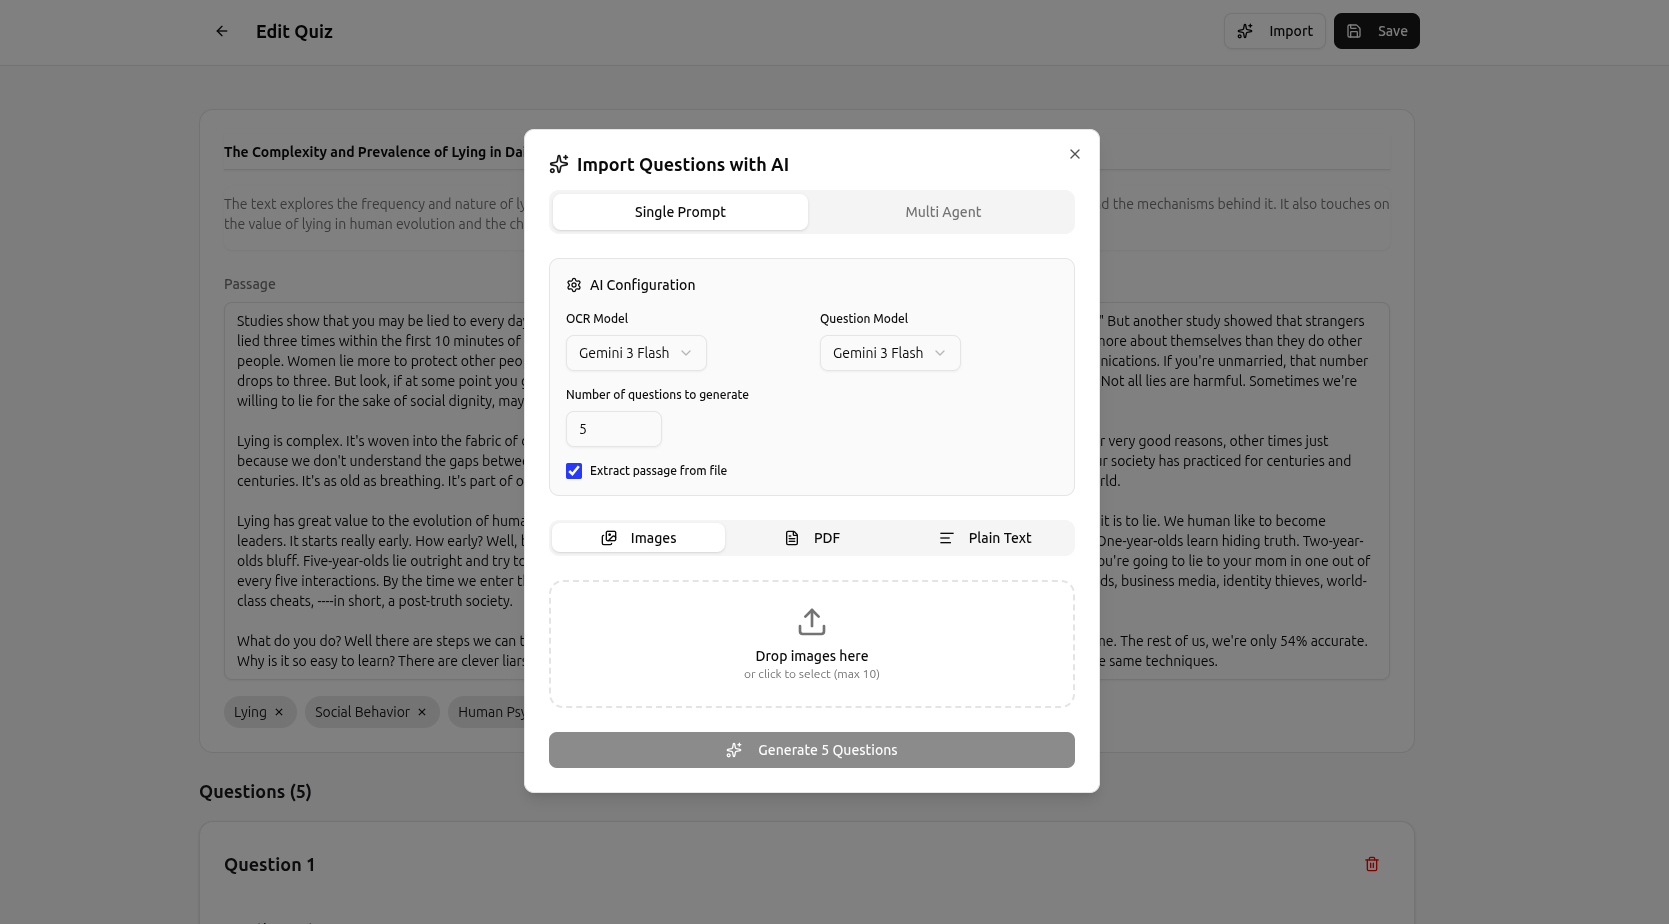
\includegraphics[width=1\linewidth]{figures/ui-edit.png}
    \caption{Giao diện trang tổng quan của ứng dụng Openlet}
    \label{fig:ui-dashboard}
\end{figure}

\textbf{Trang làm bài kiểm tra:} Giao diện dành cho học sinh được thiết kế tập trung vào trải nghiệm làm bài. Các thành phần chính bao gồm nội dung câu hỏi được trình bày rõ ràng, bốn phương án lựa chọn dạng nút bấm, thanh tiến trình hiển thị số câu đã hoàn thành trên tổng số câu hỏi, và nút điều hướng giữa các câu. Nếu giáo viên bật tính năng bộ đếm thời gian, giao diện hiển thị đồng hồ đếm ngược ở góc trên cùng với cảnh báo khi thời gian sắp hết, và có thể tự động nộp bài khi hết giờ.

\textbf{Trang kết quả:} Sau khi nộp bài, học sinh được chuyển tới trang kết quả với nội dung hiển thị tùy theo mức hiển thị mà giáo viên đã cấu hình. Ở mức cơ bản nhất, trang hiển thị điểm số tổng thể. Ở các mức cao hơn, trang bổ sung thêm thông tin chi tiết từng câu hỏi bao gồm trạng thái đúng/sai, đáp án đúng và giải thích.

\textbf{Trang thống kê:} Dành cho giáo viên, trang này cung cấp cái nhìn tổng quan về kết quả làm bài của tất cả học sinh. Các thành phần chính bao gồm biểu đồ phân phối điểm theo năm khoảng, bảng xếp hạng năm người đạt thành tích cao nhất, các chỉ số tổng hợp (điểm trung bình, cao nhất, thấp nhất, tổng số lượt làm bài) và danh sách chi tiết từng lượt làm bài với thông tin người làm, điểm số và thời gian nộp.

\begin{figure}[htbp]
    \centering
    \begin{minipage}{0.48\textwidth}
        \centering
        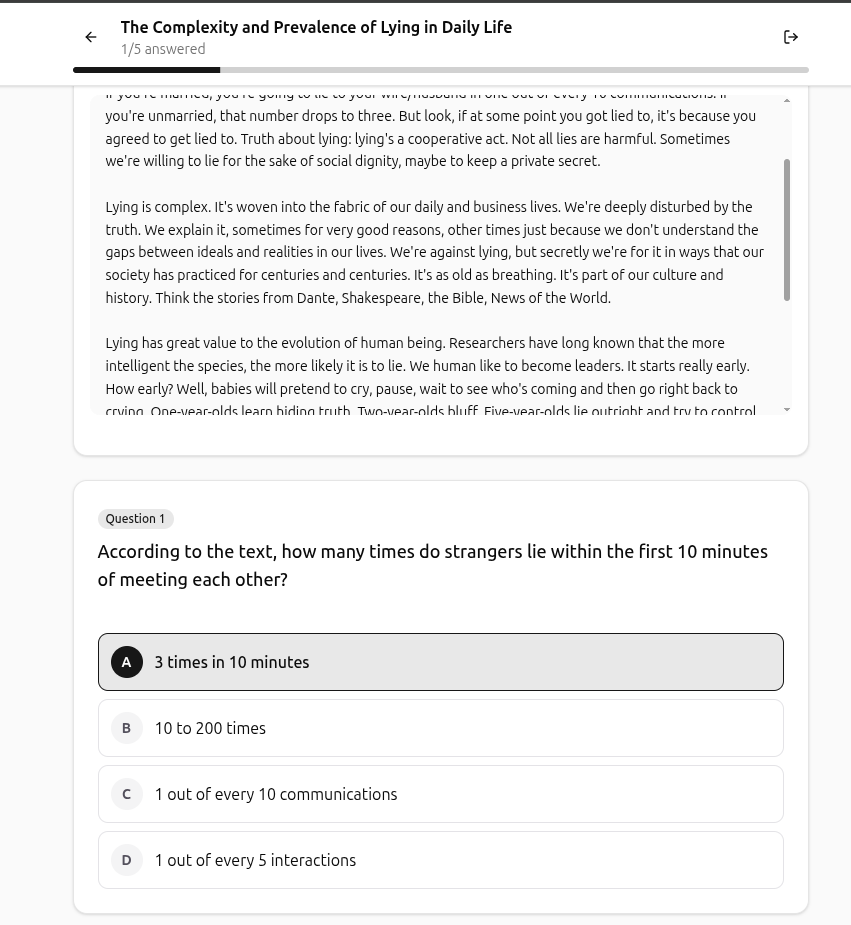
\includegraphics[width=\textwidth]{figures/ui-student-play.png}
    \end{minipage}
    \hfill % Tạo khoảng trống linh hoạt giữa 2 ảnh
    \begin{minipage}{0.48\textwidth}
        \centering
        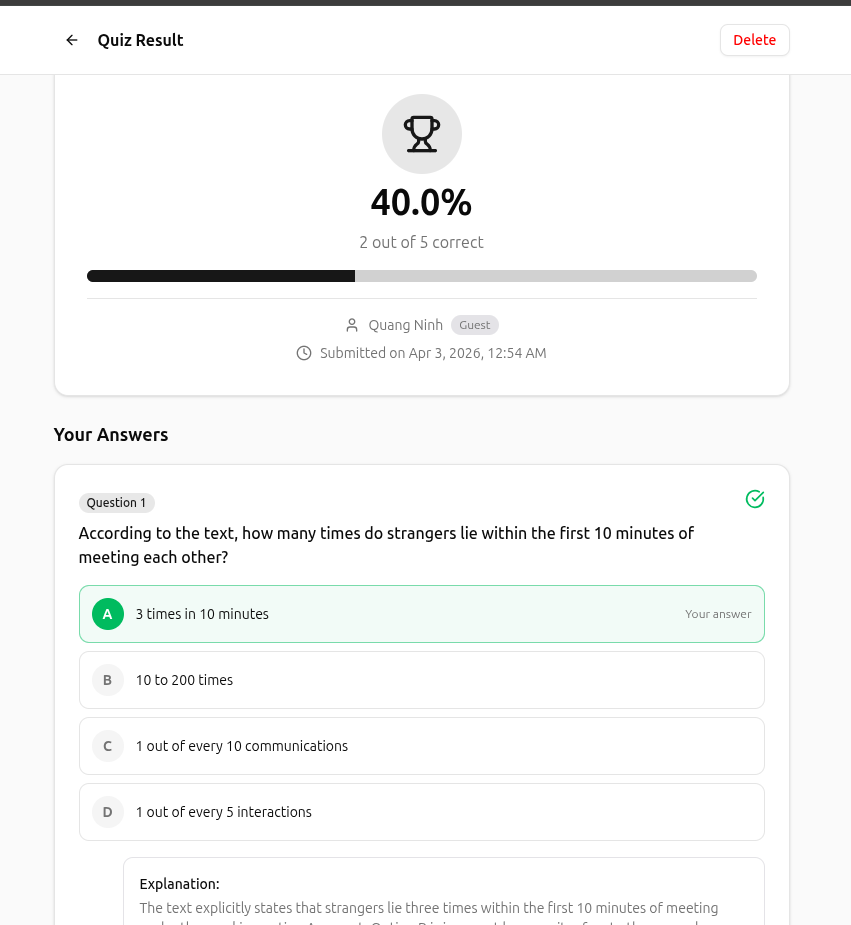
\includegraphics[width=\textwidth]{figures/ui-student-result.png}
    \end{minipage}

    \vspace{10pt} 
    \caption{Giao diện trang làm bài kiểm tra (trái) và kết quả (phải)}
    \label{fig:ui-quiz-taking}
\end{figure}

% % [NEW]: Figure placeholder cho giao dien trang ket qua va trang thong ke
% \begin{figure}[htbp]
%     \centering
%     % [Figure Suggestion]: Chen anh chup man hinh trang ket qua va trang thong ke.
%     % Trang ket qua (ben trai): hien thi diem so lon o tren, danh sach cau hoi ben duoi voi mau xanh (dung) va do (sai).
%     % Trang thong ke (ben phai): bieu do cot phan phoi diem, bang xep hang top 5, cac chi so tong hop.
%     % Co the dung 2 anh ghep ngang hoac subfigure.
%     \caption{Giao diện trang kết quả (trái) và trang thống kê (phải)}
%     \label{fig:ui-results-stats}
% \end{figure}
